\documentclass[letterpaper,12pt]{article}   %% LaTeX 2e (preferred)
\usepackage{osajnl2} %% do not use with REVTeX4
\usepackage[draft]{hyperref} %% optional
\usepackage{amsmath}
\usepackage{amssymb}
%%\usepackage{subfigure}
\usepackage{graphicx}
%%\usepackage{caption}
%%\usepackage{subcaption}
%\usepackage{setspace}
%\doublespacing


\begin{document}

\title{Improved iterative least-squares algorithm for phase-shifting
  interferometry}

\author{O. Medina,$^{1,*}$ J. C. Estrada,$^{1}$ and M. Servin,$^{1}$}

\address{$^1$Centro de Investigaciones en Optica A. C., Loma del
  bosque 115, Col. Lomas del Campestre, Leon Guanajuato, 37150,
  Mexico}

\address{$^*$Corresponding author: orlandomedina@cio.mx}

\maketitle

\begin{abstract}
  Iterative Least-Squares (ILS) algorithms are used when having a
  Phase-Shifting Interferogram (PSI) sequence where we do not know the
  inter-frame phase-shifts and these are not necessary
  constant. Basically, ILS algorithms uses the PSI least-squares model
  in two main steps: 1) Estimate the modulating phase with a set of
  guessed phase-shifts, and 2) Estimate the phase-shifts using the
  previously estimated phase. These two steps are performed
  iteratively. In this class of algorithms, a source of error is when
  is estimating the phase-shifts while the background illumination
  varies spatially. This is because the least-squares model assumes
  constant background illumination. To improve this, in this paper we
  divide in subregions the interferogram frames and apply the
  least-squares model on each subregion. Thus, each subregion may have
  its own background illumination, being less restrictive than
  applying the least-squares model to the global frame. The numerical
  experiments presented here, show that this approach enhance the
  obtained results of the well known published ILS algorithms. For
  demonstration purposes, the source code of this algorithm is
  provided in the references for download.
\end{abstract}
\ocis{120.0120, 120.3180, 120.3940, 120.5050, 120.2650, 050.5080}

\section{Introduction}
Nowadays, Phase Shifting Interferometry (PSI) techniques are some of
the most used techniques in optical metrology
\cite{a1_OpticalTesting}. In PSI, one obtains a small sequence of at
least 3 interferograms with a phase-shift among them
\cite{a1_OpticalTesting}. To recover the modulating phase, there are
standard demodulation PSI methods, the well known 3-, 4-, and 5- step
phase-shifting algorithms.  Knowing the inter-frame phase-shifts (or
temporal carrier), the standard methods recover the 2$\pi$ modulus
phase map with the minimum possible error
\cite{a1_OpticalTesting,a2_F_K,a3}. If we do not know the phase-shifts
exactly, we obtain a phase map with an unavoidable detuning error
whose magnitude depends on the number of interferograms employed and
on how far we are from the actual phase-shifts
\cite{a3,a4,a5,a6}. This unfortunate case can occur when the optical
interferometer setup is miscalibrated or when perturbations from the
environment affect the interferometer's optical path. For example, for
most phase shifters, such as a piezoelectric (PZT), there is a
repeatability problem arising from hysteresis, non linearity and
temperature linear drift \cite{a5,a7}; curiously, the first
phase-shifting algorithms were self-tuning nonlinear algorithms
\cite{a8,a9}. To reduce detuning errors, other approaches propose
error compensating algorithms that basically use redundant data, such
as the Schwider- Hariharan 5- step algorithm \cite{a4,a10,a11}, and
more recently, the 9-step algorithm shown in Ref. \cite{a12} has been
used to do it by constructing a wide-band frequency response of the
phase-shifting algorithm. Further methods use the Fourier transform in
order to estimate the inter-frame phase-shifts, and others are based
on the least-squares scheme, iteratively estimating the inter-frame
phase-shifts and phase \cite{a13,a14}.  Ref. \cite{a16} presents an
approach that estimates the local temporal carrier (the phase-shift)
as the average of the phase difference between two consecutive phase
maps obtained from two realizations of the tunable 3-step
algorithm. What we are going to show in this work is a regularized
self-tuning demodulation technique that obtains the analytical image
(complex interferogram) and inter-frame phase-shifts from an
interferogram sequence. Thus, we can recover the modulating phase
2$\pi$ modulus and the inter-frame phase shifts in the same
process. Here, it is not necessary to know the inter-frame
phase-shifts. These inter-frame phase-shifts can vary arbitrarily.

The main difference between the demodulation method presented here and
the ones reported in \cite{a14},\cite{a15} and \cite{a17} is that our
demodulation method is based on a regularization technique that is
robust to non-constant modulation variations and non-constant
background illumination, which is an issue that introduces errors in
the methods in works \cite{a14} and \cite{a15}. Besides, we do not
require to estimate the fringe orientation, as the method in work
\cite{a17}.

\section{Method}

In general, an interferogram sequence with arbitrary inter-frame
phase-shifts can be modeled as:
\begin{equation} \label{eq:I_k1}
  I_k(x,y)=a(x,y)+b(x,y)cos(\phi(x,y)+\delta_k),\quad k=0,1,2,...,L-1,
\end{equation}
where $I_k(x,y)$ is the intensity at the site $(x,y)\in\Gamma$ of the
$k$-interferogram in a sequence of $L$ interferograms; being $\Gamma$
the lattice of the interferogram's frame (frame domain), $a(x,y)$ the
background illumination, $b(x,y)$ the contrast, $\phi(x,y)$ the
modulating phase under test and $\delta_k$ the interframe phase-shift
of the $k$-interferogram.

\subsection{Iterative Least-Squares (ILS) algorithm}
Actually, ILS algorithms use two systems with the same least-squares
model. The input of the system one, is the interferogram sequence
$I_k$ and interframe phase-shifts $\delta_k$ for $k=0,1,2,\dots,L-1$;
and its output is the modulating phase $\phi(x,y)$. In system two, the
input is the $k$-interferogram $I_k$ and all sites $(x,y)$ of the
modulating phase $\phi$, and its output is the $k$-interferogram
phase-shift $\delta_k$. Thus, iteratively the system one feeds the
system two and vice versa.

The PSI least-squares model of system one for estimating the
modulating phase $\phi$ at $(x,y)$ can be written as follows:
\begin{equation}
  U_1(a_{x,y},C_{x,y},S_{x,y}) = \sum_{k=0}^{L-1}\left[
    a_{x,y}+C_{x,y}\cos(\delta_k)-S_{x,y}\sin(\delta_k)-I_k(x,y)
  \right]^2, \label{eq:ls-phase}
\end{equation} 
where $C_{x,y}=\cos[\phi(x,y)]$ and $S_{x,y}=\sin[\phi(x,y)]$ are the
unknown quadrature components of the interferogram sequence and
$a_{x,y}$ is the unknown background illumination at $(x,y)$. Thus,
minimizing Eq. \eqref{eq:ls-phase} with respect to $C_{x,y}$,
$S_{x,y}$ and $a_{x,y}$, we estimate the modulating phase $\phi(x,y)$
in the following way:
\begin{equation}
  \hat\phi(x,y) = \arctan\left[-\frac{S_{x,y}}{C_{x,y}}\right].
\end{equation}
The least-squares model of system two for estimating the
$k$-interframe phase-shift $\delta_k$ is:
\begin{equation}
  U_2(a_k,C_k,S_k) = \sum_{(x,y)\in \Gamma}\left[
    a_k+C_k\cos[\phi(x,y)]-S_k\sin[\phi(x,y)]-I_k(x,y)
  \right]^2, \label{eq:ls-steps}
\end{equation} 
where $C_k=\cos(\delta_k)$ and $S_k=\sin(\delta_k)$ are the unknowns
and the sum runs over all sites of the domain $\Gamma$. Minimizing
Eq. \eqref{eq:ls-steps} with respect to $C_k$, $S_k$ and $a_k$, we
estimate the $k$-interframe phase-shift $\delta_k$ as:
\begin{equation}
  \hat\delta_k = \arctan\left[-\frac{S_k}{C_k}\right].
\end{equation}
It is important to note the following:
\begin{itemize}
\item[1] The model of Eq. \eqref{eq:ls-phase} is for the $(x,y)$ site,
  runs over the interferograms, and assumes that the background
  illumination $a_{x,y}$ does not changes along the interferogram
  sequence.
\item[2] The model of Eq. \eqref{eq:ls-steps} is for the
  $k$-interferogram, runs over all sites of the frame, and assumes
  that the background illumination of that frame, denoted by $a_k$, is
  constant.
\end{itemize}
The assumption of Eq. \eqref{eq:ls-phase} is not so restrictive
because actually the background illumination commonly does not changes
between interferogram frames. However, the assumption of
Eq. \eqref{eq:ls-steps} is more restrictive since as stated in
Eq. \eqref{eq:I_k1}, we can not expect a constant background
illuminations of the interferogram frame.

For being more accurate with the system two (Eq. \eqref{eq:ls-steps}),
we propose divede the interferogram frame in $N$ subregions as
illustrated in Fig. \ref{fig:subregions}.
\begin{figure}
  \centering
  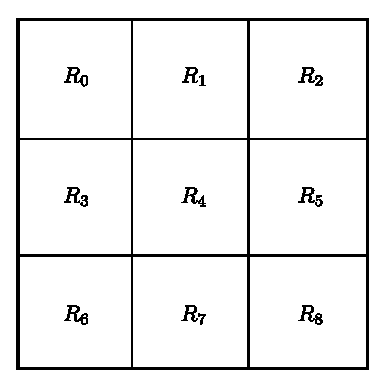
\includegraphics[width=4cm]{regions.eps}
  \caption{Subregion division of interferogram frame. In practice, an
    interferogram frame is divided into $N$ subregions where each
    subregion has the same size.\label{fig:subregions}}
\end{figure}
Then system two is applied to each subregion independently in such a
way that we are going to have $N$ estimations of the background
illumination and cuadrature components for the phase-shifts.

\bibliographystyle{plain} \bibliography{rst.bib}
\end{document}
